\documentclass[journal,twoside,10pt]{IEEEtran}

% Packages
\usepackage{cite}
\usepackage{amsmath,amssymb,amsfonts}
\usepackage{algorithmic}
\usepackage{graphicx}
\usepackage{textcomp}
\usepackage{xcolor}
\usepackage{listings}
\usepackage{afterpage}

% Custom section formatting for IEEEtran
\makeatletter
% Use Roman numerals for sections
\renewcommand\thesection{\Roman{section}}
% Format sections with Roman numerals and add period
\renewcommand\section{\@startsection{section}{1}{\z@}%
                       {-3.5ex \@plus -1ex \@minus -.2ex}%
                       {2.3ex \@plus.2ex}%
                       {\normalfont\Large\bfseries\Roman{section}.\quad}}
% Keep subsections unnumbered with no dot
\renewcommand\thesubsection{}
% Redefine subsection to avoid using any numbering
\renewcommand\subsection{\@startsection{subsection}{2}{\z@}%
                       {-3.25ex\@plus -1ex \@minus -.2ex}%
                       {1.5ex \@plus .2ex}%
                       {\normalfont\large\bfseries}}
% Empty section format to prevent automatic numbering
\renewcommand\@seccntformat[1]{}
\makeatother

% Configure listings package with enhanced JSON styling
\lstdefinestyle{mystyle}{
    backgroundcolor=\color{gray!10},
    commentstyle=\color{green!50!black},
    keywordstyle=\color{blue},
    stringstyle=\color{purple},
    basicstyle=\ttfamily\small,
    breakatwhitespace=false,
    breaklines=true,
    captionpos=b,
    keepspaces=true,
    numbers=none,
    numbersep=5pt,
    showspaces=false,
    showstringspaces=false,
    showtabs=false,
    tabsize=2
}

% Custom JSON styling
\lstdefinelanguage{JSON}{
    morestring=[b]",
    stringstyle=\color{purple},
    showstringspaces=false,
    keywords={false,true,null},
    keywordstyle=\color{orange},
    morekeywords={[2]"task_id","task","plan","actions","step","controlLabel","controlText","function","args","file_path"},
    keywordstyle={[2]\color{blue}},
    sensitive=false,
    comment=[l]{//},
    commentstyle=\color{green!50!black},
    morecomment=[s]{/*}{*/},
    literate=
        {:}{{{\color{black}{:}}}}{1}
        {,}{{{\color{black}{,}}}}{1}
        {\{}{{{\color{black}{\{}}}}{1}
        {\}}{{{\color{black}{\}}}}}{1}
        {[}{{{\color{black}{[}}}}{1}
        {]}{{{\color{black}{]}}}}{1}
}

\lstset{style=mystyle}

\begin{document}

\title{A State-of-the-Art Survey on AI Systems for Multi-Task Productivity: From Large Language Models to Multi-Agent Systems}

\author{Your Name \\ Your Affiliation}

\maketitle

\begin{abstract}
The rapid evolution of large language models (LLMs) has catalyzed the development of systems capable of performing multiple productive tasks. Early breakthroughs in language modeling paved the way for models to autonomously select and utilize external tools. Subsequent research focused on transforming these models into Large Action Models (LAMs) tailored for action execution. More recently, integrating LAMs within multi-agent systems (MASs) has emerged as a promising strategy for tackling complex, real-world tasks. This survey synthesizes historical progress, contemporary research, and future directions in the field—from LLMs using tools to MASs that achieve collaborative, autonomous task execution.
\end{abstract}

\begin{IEEEkeywords}
LLMs, Toolformer, ToolLLM, Large Action Models, Multi-Agent Systems, Autonomous Agents, Collaborative AI
\end{IEEEkeywords}

\section{Introduction}
Large language models (LLMs) have redefined what is possible in artificial intelligence, demonstrating unprecedented capabilities in natural language understanding and generation. Despite their success, early LLMs were inherently limited to text-based outputs and struggled with tasks requiring real-world action. Recent work has demonstrated that LLMs can be extended to identify and call appropriate tools, effectively bridging the gap between language and action. This survey reviews the evolution from tool-using LLMs to specialized Large Action Models (LAMs), and ultimately to multi-agent systems that harness these capabilities for collaborative, productive task execution.

In the following sections, we outline:
\begin{itemize}
    \item \textbf{How we got here:} A brief history of LLMs' transformation through tool usage.
    \item \textbf{Where we are now:} The emergence of LAMs and their integration into multi-agent frameworks.
    \item \textbf{Where we could go next:} Challenges faced by current systems and potential directions for future research.
\end{itemize}

\section{Literature Review}

\subsection{From Language Models to Tool-Using Agents}

Advancements in artificial intelligence have accelerated in recent years, particularly with the introduction of the transformer architecture. This innovation enabled commercial LLM-supported products and significantly impacted society's understanding of AI. From a product engineering perspective, where user interface design is paramount and team value comes from well-crafted experiences, the chat interface has been widely embraced. This rapid adoption is no coincidence—our first interactions with LLMs occurred through interfaces that create the impression of conversing with another person, resulting in a natural experience that increased user adoption.

Initially, the value users derived from these interfaces was largely limited to text generation. As interactions became multimodal, the term "Generative AI" become popular to describe these systems. This term reflects both their architectural approach to generating outputs and their perceived intelligence and creativity—their ability to create new ideas, images, and sounds. This framing helps us understand phenomena like "hallucinations" and other characteristics of these AI systems.

In brief, contrary to science fiction's predictions, we have developed a form of artificial intelligence that excels more at creative tasks than logical ones. This observation sets the foundation for our literature review: while current AI shows immense potential, it still lacks the reliability needed for complex task execution.

In this research exercise, we identify a trend of evolution that expands around 3 years, i.e., \cite{schick2023toolformer, qin2023toolllm}. Researchers noticed the potential of the LLMs to be used for more than just text generation, as they display excellent ability to understand and produce structured output, there was a possibility of integrate with existing software artifacts already in place, such as APIs, SDKs, and any other programmable interface.

API's where one of the most natural places to start with.  Toolformer (Schick et al., 2023)~\cite{schick2023toolformer} represents a breakthrough in addressing LLM limitations through tool integration, enabling models to autonomously determine when external tools are needed, select appropriate ones, and incorporate their outputs into ongoing language generation. Its distinctive self-supervised learning methodology implements a streamlined three-step process that samples potential API calls using in-context learning, executes these calls to obtain results, and filters them based on perplexity reduction. This approach creates a more adaptive system capable of determining which tools benefit specific contexts without extensive human annotation.

Expanding this line of research, ToolLLM (Qin et al., 2023)~\cite{qin2023toolllm} introduces a comprehensive framework for training models to effectively utilize external tools through API calls. It contributes three key innovations: a systematic methodology for converting conventional dialogue datasets into tool-use examples through automated annotation; ToolBench, a diverse dataset spanning over 16,000 real-world scenarios across various domains; and a training approach enabling models to make effective API calls without human intervention. Performance evaluations demonstrate that tool-augmented models significantly outperform standard approaches, particularly in generating syntactically correct API calls, tool selection, and output integration.

These complementary innovations mark a crucial first step in improving the reliability of AI systems for performing specific tasks by establishing a new paradigm where language models can handle tasks beyond linguistics to perform useful, real-world operations. By maintaining sophisticated language understanding while gaining access to specialized functionality, tool-augmented systems offer a cost-effective approach to enhancing model capabilities without increasing model size, potentially transforming how AI assistants support human productivity across diverse domains.

\subsection{Large Action Models (LAMs)}
While tool-using LLMs represent an important breakthrough, many applications require systems that can perform actions in dynamic environments rather than merely generating text. This led to the development of Large Action Models (LAMs), which are fine-tuned to execute tasks \cite{wang2025lam}.

\subsubsection{Developing and Training Large Action Models}

Creating effective LAMs requires a systematic development pipeline that transforms a general-purpose language model into a specialized action execution system. Drawing on the insights from Wang et al.~\cite{wang2025lam}, this process encompasses several interconnected stages:

\paragraph{Data Collection and Preparation}
The foundation of LAM development lies in gathering and curating task-specific data. This initial phase follows a two-phase approach:

\begin{itemize}
    \item \textbf{Task-Plan Data Collection:} This involves collecting user requests and corresponding step-by-step plans. Sources include application documentation, WikiHow articles, and historical search queries. Each entry typically contains a task description and a detailed plan outlining the steps required to accomplish it.
    
    \item \textbf{Task-Action Data Collection:} This phase converts task-plan data into executable task-action data. Each plan step is transformed into concrete, actionable instructions that can be directly executed in the target environment. This process includes instantiation (adding specific operational details), execution validation, and evaluation to ensure correctness.
\end{itemize}

For example, a typical task-plan data entry might look like:

\begin{lstlisting}[language=JSON]
{
  "task_id": "powerpoint_task_001",
  "task": "Create a slide based on draft.docx",
  "plan": [
    "1. Open the draft.docx and read the content.",
    "2. Create a new PowerPoint file.",
    "3. For page 1, add ..."
  ]
}
\end{lstlisting}

While a corresponding task-action entry would include additional execution details:

\begin{lstlisting}[language=JSON]
{
  "task_id": "powerpoint_task_001",
  "task": "Create a slide based on draft.docx",
  "plan": [...],
  "actions": [
    {
      "step": "open the document",
      "controlLabel": "",
      "controlText": "",
      "function": "open",
      "args": {"file_path": "draft.docx"}
    }
  ]
}
\end{lstlisting}

\paragraph{Training an LLM into a LAM: A Four-Phase Approach}

\begin{figure}[htbp]
    \centering
    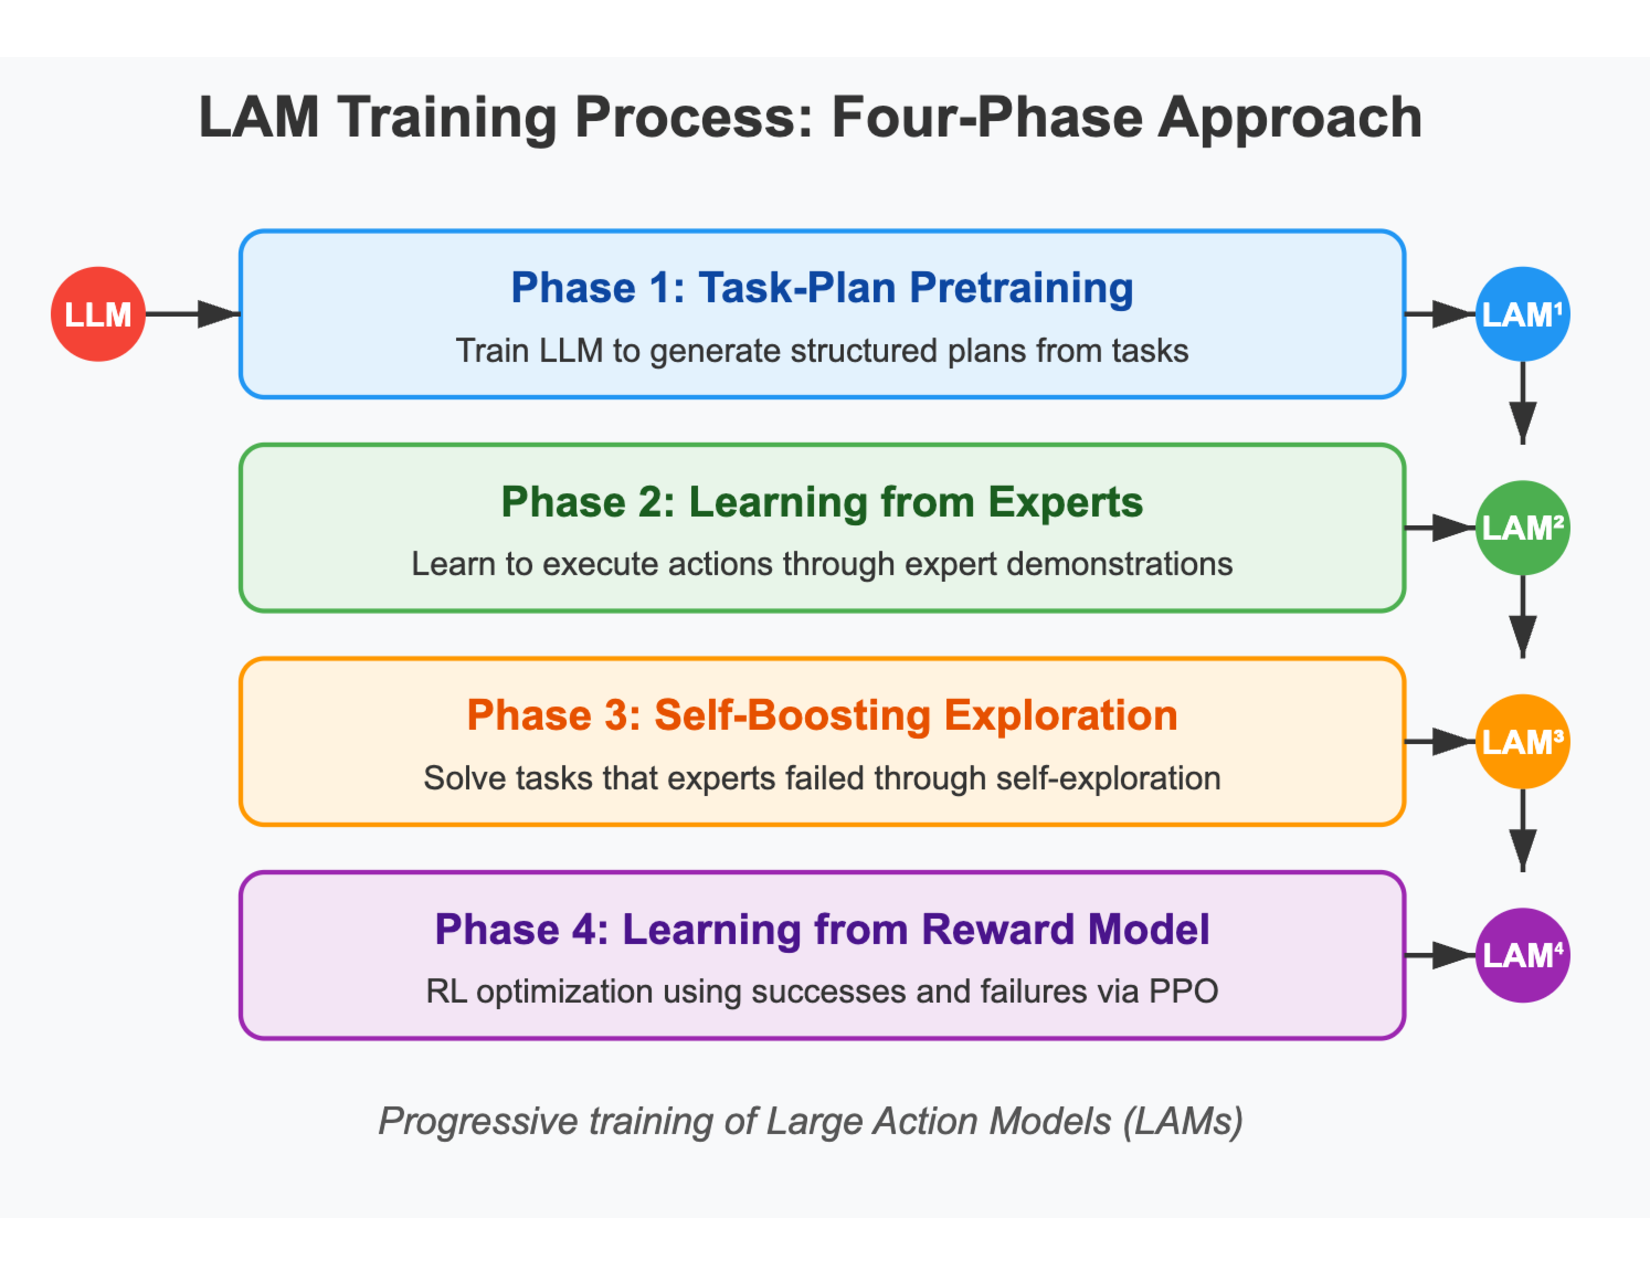
\includegraphics[width=0.5\textwidth]{traning_phases.pdf}
    \caption{Progressive four-phase training approach for transforming a general LLM into a specialized LAM.}
    \label{fig:lam-training}
\end{figure}

The transformation of a general-purpose language model into a specialized Large Action Model represents the technical core of LAM development. Wang et al. \cite{wang2025lam} propose a systematic, four-phase training process that progressively builds capabilities from planning to action execution:

\begin{enumerate}
    \item \textbf{Task-Plan Pretraining:} In this foundational phase, the model (LAM$^1$) learns to generate structured, step-by-step plans for completing tasks. Using supervised fine-tuning with task-plan pairs, the model develops the ability to break tasks into logical sequences. At this stage, the model can generate coherent plans but lacks execution capabilities.
    
    \item \textbf{Learning from Experts:} In the second phase, the model (LAM$^2$) learns to translate plans into concrete, executable actions through expert demonstrations. Training uses state-action pairs where each state includes the current UI environment and task context, and each action specifies which control to interact with and how. This phase grounds the model's reasoning in real application environments.
    
    \item \textbf{Self-Boosting Exploration:} Moving beyond expert-only training, the third phase introduces self-improvement. LAM$^2$ attempts tasks that experts (like GPT-4o) failed to solve, generating new successful trajectories. These self-discovered solutions, combined with original expert demonstrations, create an augmented dataset used to train LAM$^3$. This represents a critical step toward greater model autonomy.
    
    \item \textbf{Learning from a Reward Model:} The final phase introduces reinforcement learning, enabling the model to learn from both successes and failures. First, a reward model is trained on both successful and failed trajectories, assigning positive values to successful steps and negative values to failures. Then, LAM$^4$ is fine-tuned using Proximal Policy Optimization (PPO) on previously failed trajectories, guided by the reward model's feedback. This approach significantly enhances the model's decision-making abilities in complex scenarios.
\end{enumerate}

Throughout this progressive training approach, each phase builds upon previous ones, creating increasingly capable systems that combine high-level planning, expert-guided execution, autonomous exploration, and reward-based optimization.

\paragraph{Integration and Grounding}
Once trained, the LAM must be integrated into an agent framework to interact with real-world environments:

\begin{itemize}
    \item \textbf{Environment Interface:} Mechanisms to observe and interact with the target environment, such as UI Automation APIs that provide information about actionable controls.
    
    \item \textbf{Action Execution:} Systems to translate model outputs into tangible actions within the environment, mapping predicted actions to specific function calls.
    
    \item \textbf{Memory Management:} Components to maintain historical actions and plans, providing essential context for future decisions and enabling more coherent multi-step execution.
    
    \item \textbf{Feedback Loops:} Structures to collect environmental responses and adapt accordingly, allowing the agent to respond to changing conditions.
\end{itemize}

\paragraph{Evaluation}
The final stage involves rigorous assessment of the LAM's performance:

\begin{itemize}
    \item \textbf{Offline Evaluation:} Testing on controlled datasets without environmental interaction, measuring metrics like Task Success Rate, Object Accuracy, and Operation Accuracy.
    
    \item \textbf{Online Evaluation:} Deploying the model in real environments to measure practical performance, including Task Completion Time and Average Step Latency—crucial for assessing real-world applicability.
\end{itemize}

This comprehensive development pipeline ensures that LAMs can effectively translate user intentions into meaningful actions within specific operational contexts. Each stage contributes essential capabilities, culminating in models that can perform complex, multi-step tasks in real-world environments—representing a fundamental advancement over traditional language models limited to text generation.

\subsubsection{Applications and Impact}
LAMs enable a wide range of applications previously challenging for traditional LLMs, including:

\begin{itemize}
    \item Autonomous interaction with software applications and operating systems
    \item Control of physical devices and robotic systems
    \item Complex task automation in specialized domains like healthcare or finance
    \item Multi-step problem-solving that requires environmental awareness
\end{itemize}

These capabilities mark a significant advancement toward artificial general intelligence (AGI), enabling AI systems to automate tasks that were previously only possible with human intervention.

LAMs thus represent a paradigm shift—from language generation to action execution—allowing AI systems to automate complex processes with minimal human intervention, substantially expanding their practical utility across numerous domains.

\subsection{Multi-Agent Systems}

\begin{figure}[htbp]
    \centering
    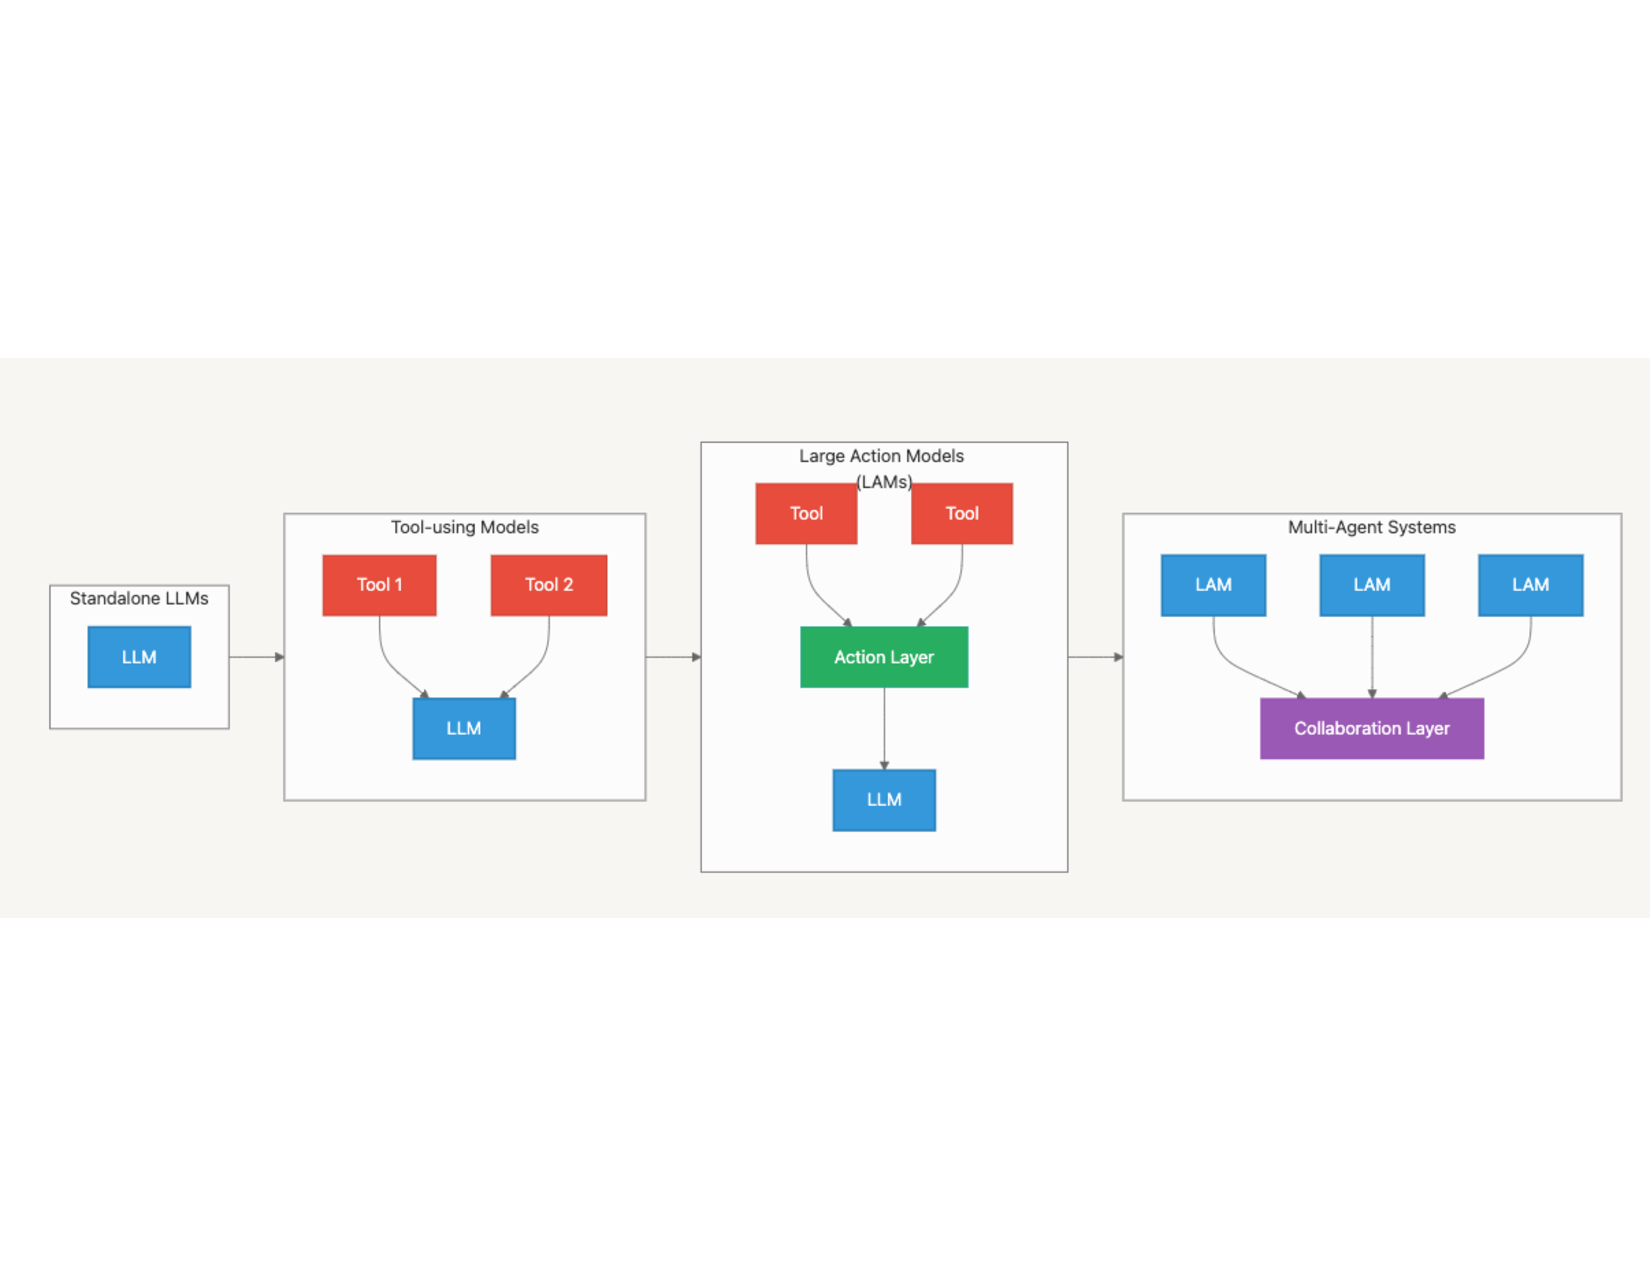
\includegraphics[width=0.5\textwidth, trim=0 150pt 0 150pt, clip]{lams_diagram.pdf}
    \caption{Evolution of AI systems from standalone LLMs to multi-agent systems.}
    \label{fig:lam-evolution}
\end{figure}

The integration of Large Action Models (LAMs) into multi-agent systems (MASs) represents the next frontier in AI system design~\cite{tran2025multiagent}. While LAMs enable individual AI systems to execute actions in the real world, their true potential emerges when multiple such agents collaborate to accomplish tasks that exceed the capability of any single agent. This collaborative approach fundamentally transforms how AI operates by shifting from isolated models toward interconnected systems that can distribute complex problems, dynamically allocate resources, and achieve higher levels of robustness through redundancy.

At their core, LLM-based multi-agent systems consist of multiple interacting intelligent entities, each potentially powered by a LAM. Every agent operates with its own language model serving as its cognitive "brain," specialized memory and knowledge base, defined objectives guiding its actions, environmental awareness providing context, and action capabilities enabled through LAM integration. The connective tissue between these agents—the collaboration channels—enables them to communicate, coordinate, and collectively tackle complex, multi-step challenges.

The collaboration mechanisms in these systems can take various forms. In cooperative scenarios, agents align their individual objectives with shared goals, often specializing in complementary roles to enhance efficiency. This approach has proven successful in applications ranging from question answering to collaborative programming, where different agents may handle research, planning, execution, and evaluation tasks. By contrast, competitive collaboration occurs when agents operate with potentially conflicting objectives, which can drive innovation and robustness through evolutionary pressure. Such competition-based approaches have shown benefits in debate frameworks and strategic gaming environments, where contradictory perspectives often yield more nuanced and comprehensive solutions. A hybrid approach—coopetition—enables agents to collaborate on certain tasks while competing on others, facilitating negotiation and compromise in complex, multi-objective problems.

The communication structure of these multi-agent systems further defines how information flows between collaborating agents. In centralized architectures, communication follows a hub-and-spoke model where interactions flow through a central coordinator agent that manages task allocation and synthesizes results. Decentralized structures enable peer-to-peer interactions without centralized control, offering greater resilience against single points of failure but requiring more sophisticated coordination mechanisms. Hierarchical arrangements create layered structures with defined authority levels, balancing control and flexibility across different tiers of agents with varying specializations.

The coordination protocols governing these interactions range from rule-based approaches with predefined interaction guidelines to role-based systems that divide labor according to agent specialization, and model-based frameworks that adapt probabilistically to environmental uncertainty. Such protocols ensure that agent collaborations remain coherent, efficient, and aligned with overall system objectives.

By leveraging LAMs within multi-agent frameworks, these systems gain several critical advantages. Complex tasks can be decomposed and allocated across specialized agents, with each focusing on subtasks aligned with its particular strengths. Resources can be dynamically allocated based on agent expertise and availability, allowing the system to adapt to changing requirements. The inherent redundancy in agent capabilities ensures resilience when individual components fail, while the collective intelligence that emerges from these collaborations often exceeds what any single agent could achieve independently. Moreover, these systems can scale by integrating new agents with specialized functions as requirements evolve.

This integration marks a significant leap in AI system design, enabling sophisticated real-world applications where agents interact, negotiate, and cooperate autonomously. From software development teams where different agents handle specification, coding, testing, and documentation, to creative content generation where specialized agents contribute different aspects of the creative process, to research assistance and complex decision-making scenarios, LAM-powered multi-agent systems are expanding the boundaries of what AI can accomplish.

Despite their promise, these systems face important challenges that ongoing research must address. Coordination complexity increases substantially as more agents join the system, requiring sophisticated mechanisms to ensure coherent task allocation and planning. Communication overhead must be carefully balanced against the benefits of collaboration to maintain computational efficiency. Error propagation presents another concern, as individual agent mistakes can potentially cascade through the system without proper safeguards. Finally, comprehensive evaluation metrics and benchmarks for assessing multi-agent performance remain underdeveloped compared to those for single-agent systems.

As research in this field advances, addressing these challenges will be crucial for realizing the full potential of multi-agent systems in productive AI applications. The trajectory from language models to action-capable agents to collaborative multi-agent systems represents not merely an incremental improvement but a fundamental paradigm shift in how AI systems can perceive, reason, and act in the world.

\subsection{Applications and Use Cases}
Recent studies have demonstrated practical applications of these advances:

\begin{itemize}
    \item \textbf{xLAM – A Family of Large Action Models:} The xLAM series exemplifies how LAMs can empower AI agent systems \cite{zhang2024xlam}. These models, spanning various sizes and architectures, have been shown to excel in executing real-world tasks, including tool use and interactive operations.
    \item \textbf{LLM-based Multi-Agent Systems: Techniques and Business Perspectives:} This work bridges the gap between academic research and practical applications \cite{yang2024llmbased}, discussing dynamic task decomposition, proprietary data preservation, and monetization strategies.
\end{itemize}

Together, these efforts illustrate the maturation of AI systems from isolated language models to integrated, action-capable multi-agent frameworks.

\section{Future Directions}
Despite these impressive advances, several challenges remain that point to important future research directions:

\begin{itemize}
    \item \textbf{Coordination and Planning:} Ensuring effective task allocation and dynamic planning across multiple agents remains an open problem, as discussed in studies on multi-agent systems' challenges~\cite{han2024llm}.
    \item \textbf{Memory and Context Management:} Maintaining coherent shared context and memory in MASs is critical to prevent cascading errors and ensure reliable performance.
    \item \textbf{Scalability and Robustness:} As systems grow in complexity, efficient scaling and robust fault tolerance become increasingly important.
    \item \textbf{Ethical and Safety Considerations:} The deployment of autonomous agents in real-world environments requires careful attention to safety, accountability, and ethical implications.
\end{itemize}

Future research may focus on developing standardized frameworks for inter-agent communication, enhancing real-time adaptability, and integrating advanced security measures. Addressing these challenges will be key to realizing the full potential of AI systems capable of performing multiple productive tasks.

\section{Conclusion}
The evolution from LLMs to tool-using models, and ultimately to Large Action Models integrated within multi-agent systems, represents a fundamental shift in AI capabilities. By transitioning from passive text generation to active task execution, these systems are poised to transform numerous domains—from automated workflows to complex collaborative applications. While significant progress has been made, further research into coordination, scalability, and safety is essential to fully harness the power of these intelligent systems.

\bibliographystyle{IEEEtran}
\bibliography{references}
 

\end{document}